\documentclass{templateNote}
\usepackage{tcolorbox}
\usepackage{hyperref}
\usepackage{amsmath}
\usepackage{amssymb}
\usepackage{array}
\usepackage{soul}
\usepackage{circuitikz}
\usepackage{float}
\usepackage[inline]{enumitem}
\usepackage{multicol}
\usepackage{colortbl}
\usepackage{tikz}
\usepackage{xcolor}
\usepackage[table]{xcolor}



\begin{document}
\imagenlogoU{img/logoNGMFormal_sinF.png}
\linklogoU{https://github.com/NicoGomezM} 
% \imagenlogoD{img/logo-ubb-txt-face.png} 
\titulo{Certamen 3}
\asignatura{Administración y programación de base de datos}
\autor{
    \indent
    Nicolás {Gómez Morgado}
}


\portada
\margenes 
% \tableofcontents
% \newpage


\section{Ejercicios}

\begin{enumerate}
    \item Supongamos que estamos utilizando un sistema de disco donde el tiempo para mover la cabeza de lectura/escritura a un bloque de 15ms, y el tiempo de transferencia de un bloque es de 0.4ms. Supongamos que queremos calcular el join de R con S, y tenemos que B(R)=1000, B(S)=500 y M=101. Para acelerar el join, queremos leer y escribir tantos bloques como podamos en posiciones consecutivas del disco, y usar buffers que puedan ser múltiplos de un bloque. Responda las siguientes preguntas. \\\\
    Tiempo en mover cabeza a un bloque: 15ms.\\
    Tiempo transferencia de un bloque: 0.4ms \\
    \underline{$R \Join S$}\\
    \hspace*{0.25cm} B(R) = 1000 \\
    \hspace*{0.25cm} B(S) = 500 \\
    \hspace*{0.25cm} M = 101 $\rightarrow$ 100 (Se deja uno para la salida)\\
    \begin{enumerate}[label=\alph*)]
        \item ¿Cuantas E/S de disco se requieren para realizar esta operación join? \\

        \begin{tabular}{|m{2cm}|m{6cm}|m{4cm}|}
            \hline
            $1^{er}$ pasada & Leer M bloques de R en MP[Memoria principal] (ordenar, escribir contenido ordenando) & 2B(R) crear sublistas ordenadas \\
            \hline
            $2^{da}$ pasada & El atributo de ordenación y unión & B(R) leer cada sublista \\
            \hline
            & Total & 3B(R) \\
            \hline
        \end{tabular}
        
        \vspace{0.5cm}
        \noindent Que para R son 3B(R), por lo tanto para S, es lo mismo 3B(S). \\Se rquiere B(R) + B(S). \\

        \textbf{Total: }\\
        Lo mismo para S $\rightarrow$ 3B(S) App. requerimientos [$\sqrt[]{{B(R)+B(S)}}$]\\
        \begin{align*}
            \textnormal{Disco E/S} &= 3(B(R)+B(S)) \\
            &= 3(1000+500) \\
            &= 4500 \\ 
        \end{align*}
        Por lo tanto son necesarias 4500 E/S de disco para realizar la union.\\

        \item ¿Cuanto tiempo toma un join basado en ordenamiento (sort-merge join), suponiendo que escribimos sublistas ordenadas en bloques consecutivos del disco? \\\\
        Sublista de R = $\frac{B(R)}{100} = \frac{1000}{100}$ = 10 \\
        Sublista de S = $\frac{B(S)}{100} = \frac{500}{100}$ = 5 \\

        \begin{tabular}{|m{2cm}|m{10cm}|}
            \hline
            $1^{er}$ pasada & R (Lectura y escritura) y S (Lectura y escritura): misma pista de lectura/escritura secuenciales \\
            \hline
            & $[15+(10)\cdot[(100\cdot4)+(100\cdot4)]]+[15+(5\cdot[(100\cdot4)+(100\cdot4)])]$ \\ 
            & $[15+(10)\cdot[80]]+[15+(5\cdot[80])]$ \\
            & $[15+800]+[15+400]$ \\
            & $815+415$ \\
            & 1230 ms. \\
            \hline
        \end{tabular}

        \begin{tabular}{|m{2cm}|m{6cm}|m{6cm}|}
            \hline
            $2^{da}$ pasada & Original \newline 15 buffers c/u con 1 bloque & Nueva: 15 buffers c/u con 6 bloques\\
            \hline
            & 15 buffers $\cdot$ 15 ms & 17 times $\cdot$ 15 buffers $\cdot$ 15 ms \\
            & = 100 times $\cdot$ 15 buffers $\cdot$ 15 ms & $\backsim$ 3825 ms \\
            & = 25500 ms = 22.5 seg & $\backsim$ 3.825 seg\\
            \hline
        \end{tabular}
        
        \begin{align*}
            1 \textnormal{ buffer} - 1 \textnormal{ bloque} &= 1230 ms + 22500 ms = 23730 ms \approx 23.7 seg.\\ %TODO:Destacar de azul
            1 \textnormal{ buffer} - 6 \textnormal{ bloques} &= 1230 ms + 3825 ms = 5055 ms \approx 5.05 seg.\\ %TODO:Destacar de rojo
        \end{align*}
    \end{enumerate}

    \item Supongamos que tenemos las relaciones $R(a,b)$ , $S(b,c)$ , $T(c,d)$ , $U(d,e)$ con las siguientes características:\\
        
        \begin{center}
            \begin{minipage}{0.3\textwidth}
                T(R) = 100 \\
                V(R,b) = 100 \\
                T(S) = 100 \\
                V(S,b) = 100 \\
                V(S,c) = 10 \\
                \end{minipage}%
                \begin{minipage}{0.3\textwidth}
                T(T) = 100 \\
                V(T,c) = 10 \\
                V(T,d) = 100 \\
                T(U) = 100 \\
                V(U,d) = 100 \\
            \end{minipage}
        \end{center}    

        \noindent Computar un orden de Join de R sobre S Sobre T Sobre U [$R \Join S \Join T \Join U$], utilizando:

        \begin{enumerate}[label=\alph*)]
            \item Dinámica (Dynamic Programming method) \\
            
                \begin{center}
                    \begin{tabular}{|c|c|c|c|}
                        \hline
                        R & S & T & U \\
                        \hline
                        100 & 100 & 100 & 100 \\
                        \hline
                        0 & 0 & 0 & 0 \\
                        \hline
                        R & S & T & U \\
                        \hline
                    \end{tabular}
                \end{center}

                Considerando los pares: \\

                1) $R \Join S = 100$ \\
                2) $R \Join T = 10000$ \\
                3) $R \Join U = 10000$ \\
                4) $S \Join T = 1000$ \\
                5) $S \Join U = 10000$ \\
                6) $T \Join U = 100$ \\

                \begin{center}
                    \begin{tabular}{|c|c|c|c|c|c|c|}
                        \hline
                        & R,S & R,T & R,U & S,T & S,U & T,U\\
                        \hline
                        Size & 100 & 10000 & 10000 & 1000 & 10000 & 100 \\
                        \hline
                        Cost. & & & & & &  \\
                        \hline
                        Best plan & & & & & &  \\
                        \hline
                    \end{tabular}
                \end{center}
                
                \noindent Ahora considerar la unión de 3 de las 4 relaciones. Elegir 2 para unir primero.\\
                \begin{center}
                    {R,S,T}{R,S,U}{R,T,U}{S,T,U}
                \end{center}

                1) (R,S,T) = \\
                \hspace*{0.25cm}$R \Join S = 100  \leftarrow$ \\
                \hspace*{0.25cm}$R \Join T = 10000$ \\
                \hspace*{0.25cm}$S \Join T = 1000$ 
                \begin{align*}
                    T((R \Join S) \Join T) &= \frac{T(R \Join S)\cdot T(T)}{\max\{V(R \Join S,c),V(T,c)\}} = \frac{100\cdot100}{max\{10,10\}} \\ 
                    &= \frac{10000}{10} = 1000 
                \end{align*}
                
                2) (R,S,U) = \\
                \hspace*{0.25cm}$R \Join S = 100 \leftarrow$ \\
                \hspace*{0.25cm}$R \Join U = 10000$ \\
                \hspace*{0.25cm}$S \Join U = 10000$ \\

                \hl{NIIDEA}
                \begin{align*}
                    T((R \Join S) \Join U) &= \frac{T(R \Join S)\cdot T(U)}{\max\{V(R \Join S,c),V(U,c)\}} = \frac{1000\cdot100}{max\{10,10\}} \\ 
                    &= \frac{100000}{10} = 10000
                \end{align*}
                
                3) (R,T,U) = \\
                \hspace*{0.25cm}$R \Join T = 10000$ \\
                \hspace*{0.25cm}$R \Join U = 10000$ \\
                \hspace*{0.25cm}$T \Join U = 100 \leftarrow$

                \begin{align*}
                    T((R \Join T) \Join U) &= \frac{T(R \Join T)\cdot T(U)}{\max\{V(R \Join T,d),V(U,d)\}} = \frac{10000\cdot100}{max\{100,100\}} \\ 
                    &= \frac{1000000}{100} = 10000
                \end{align*}

                4) (S,T,U) = \\
                \hspace*{0.25cm}$S \Join T = 1000$ \\
                \hspace*{0.25cm}$S \Join U = 10000$ \\
                \hspace*{0.25cm}$T \Join U = 100 \leftarrow$

                \begin{align*}
                    T((S \Join T) \Join U) &= \frac{T(S \Join T)\cdot T(U)}{\max\{V(S \Join T,d),V(U,d)\}} = \frac{1000\cdot100}{max\{100,100\}} \\ 
                    &= \frac{100000}{100} = 1000
                \end{align*}

                \begin{tabular}{|c|c|c|c|c|}
                    \hline
                    & RST & RSU & RTU & STU \\
                    \hline
                    S & 1000 & 10000 & 10000 & 1000 \\
                    \hline
                    C & 100 & 100 & 100 & 100  \\
                    \hline
                    P & $(R \Join S) \Join T$ & $(R \Join S) \Join U$ & $(T \Join U) \Join R$ & $(T \Join U) \Join S$ \\
                    \hline
                \end{tabular}
                
                \newpage
                \noindent Tripletes. \\Considerar arboles. \\

                \begin{figure}[H]
                    \centering
                    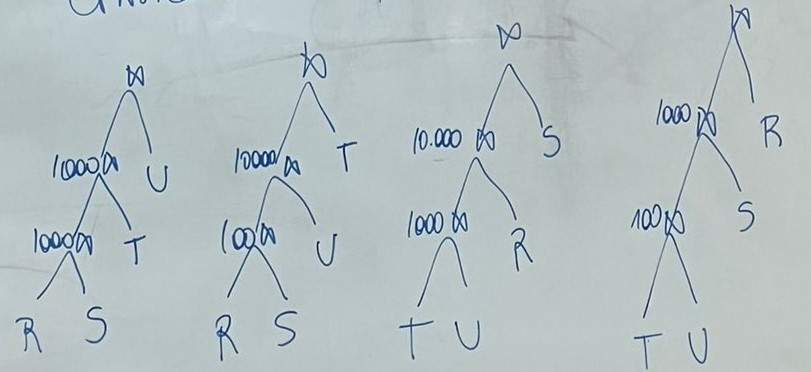
\includegraphics[width=\textwidth]{img/Imagen de WhatsApp 2024-07-08 a las 15.29.31_93439903.jpg}
                \end{figure}
                
                \noindent \textbf{Agrupando:} \\
                \begin{math}
                    (((R \Join S ) \Join T ) \Join U) = 1000 + 100 = \tikz[baseline=(char.base)]{\node[shape=circle,draw,inner sep=2pt] (char) {$1100$};} \\
                    (((R \Join S ) \Join U ) \Join T) = 10000 + 100 = 10100 \\
                    (((R \Join T ) \Join U ) \Join S) = 10000 + 100 = 10100 \\
                    (((S \Join T ) \Join U ) \Join R) = 1000 + 100 = \tikz[baseline=(char.base)]{\node[shape=circle,draw,inner sep=2pt] (char) {$1100$};} \\
                \end{math}

                \begin{figure}[H]
                    \centering
                    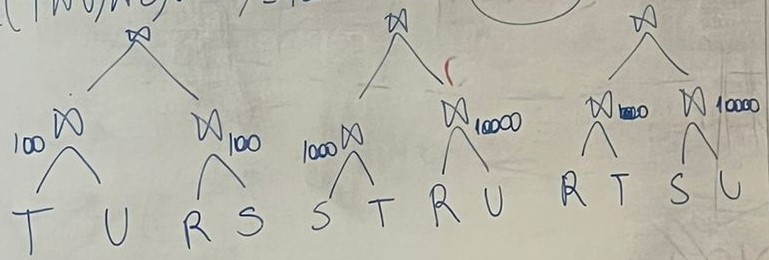
\includegraphics[width=\textwidth]{img/Imagen de WhatsApp 2024-07-08 a las 15.29.32_c3dfc849.jpg}
                \end{figure}

                \noindent \textbf{Agrupando:} \\
                \begin{math}
                    (T \Join U) \Join (R \Join S) = 100 + 100 = 200 \leftarrow\\
                    (S \Join U) \Join (R \Join U) = 10000 + 1000 = 11000 \\
                    (R \Join T) \Join (S \Join U) = 10000 + 10000 = 20000 \\
                \end{math}

            \newpage
            \item Greedy method\\
            \noindent \textbf{Se toma una decision sin retroceder.} \\
            \noindent \underline{Base:} Pares de relaciones cuyo tamaño estimado es el mas pequeño (árbol actual).

            \noindent % Evita la indentación en la primera línea
            \begin{center}
            \begin{minipage}{0.3\textwidth}
            \begin{align}
                {R,S} &= 100 \\
                {R,T} &= 10000 \nonumber \\
                {R,U} &= 10000 \nonumber 
            \end{align}
            \end{minipage}%
            \begin{minipage}{0.3\textwidth}
            \begin{align}
                {S,T} &= 10000 \nonumber \\
                {S,U} &= 10000 \nonumber \\  
                {T,U} &= 100 
            \end{align}
            \end{minipage}   
            \end{center}

            \vspace{0.5cm}
            \noindent Inducción: Encontrar todas las relaciones no includes, en este caso, T y U.

            \begin{align*}
                R \Join S &- ((R \Join S) \Join U) = 10000 \\
                R \Join S &- ((R \Join S) \Join T) = 1000 \\
            \end{align*}
            
            Se escoge T. Luego hay que unirse a U, no hay mas opciones.
            \begin{align*}
                (((R \Join S)\Join T)\Join U) = 1100
            \end{align*}

            \begin{figure}[H]
                \centering
                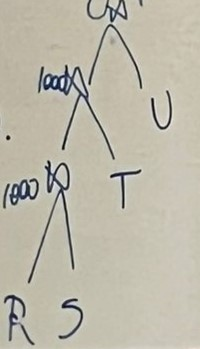
\includegraphics[width=5cm]{img/Imagen de WhatsApp 2024-07-08 a las 15.29.34_080aad61.jpg}
            \end{figure}

        \end{enumerate}

\end{enumerate}


\end{document}